\chapter{Experiments and results}

\section{Dataset}

The dataset used in this thesis is composed of video coming from smartphones and tablets with operating system \emph{Android} and \emph{iOS}. 
Videos that have an \emph{Android} acquisition device have a file container that follows the standard of the MP4 \cite{mp4} file format while videos that have an \emph{iOS} acquisition device have a file container that follows the standard of the MOV file format \cite{mov}.
The full list of devices of our dataset can be seen from Table \ref{devices}). 

\begin{table}[]
\centering
\begin{tabular}{|l|l|l|l|}
\hline
\textbf{OS}       & \textbf{BRAND}    & \textbf{MODEL}             & \textbf{\#}			 \\ \hline
Android &         &                   & 150         \\ \hline
        & Samsung &                   & 132         \\ \hline
        &         & Galaxy S3         & 18          \\ \hline
        &         & Galaxy S3 mini    & 36          \\ \hline
        &         & Galaxy S4 mini    & 18          \\ \hline
        &         & Galaxy Tab 3      & 36          \\ \hline
        &         & Galaxy Tab A      & 9           \\ \hline
        &         & Galaxy Trend Plus & 15          \\ \hline
        & Huawei  &                   & 18          \\ \hline
        &         & G6                & 18          \\ \hline
iOS     &         &                   & 110         \\ \hline
        & Apple   &                   & 110         \\ \hline
        &         & iPad 2            & 15          \\ \hline
        &         & iPad mini         & 15          \\ \hline
        &         & iPhone 4S         & 14          \\ \hline
        &         & iPhone 5C         & 18          \\ \hline
        &         & iPhone 5          & 31          \\ \hline
        &         & iPhone 6          & 17          \\ \hline
        &         &                   & 260         \\ \hline

\end{tabular}
\caption{The list of devices in the dataset divided by operating system, brand and model.}
\label{devices}
\end{table}


For each device, we have videos that are directly acquired and the same videos that have been modified by different means:

\begin{itemize}
\item videos that have been uploaded and then downloaded from 	\emph{Youtube}.
\item videos that have been modified using the software tool \emph{Ffmpeg} \cite{}.
\item videos that have been modified using the software tool \emph{Exiftool} \cite{}.
\end{itemize}

\section{Integrity Verification based on File Container}

In order to determine how our approach performs with regard to Integrity Verification we have set up some experiments. A copy of the videos in our dataset have been modified through different means, thus losing their integrity. In this experiments we check whether the information of the file containers are sufficient to tell the original videos and the modified ones apart.

The tools that we have used to modify the videos are \emph{Ffmpeg} and \emph{Exiftool}. The modification we have made are as minimal as the tools allow.

In general the experiments have been performed as follow. Given a list of videos $(x_{1},\ldots,x_{n}) \in C_{i}$, with $C_{i}$ a certain device, we have generated a corresponding list of minimally processed videos $(\overline{x_{1}},\ldots,\overline{x_{n}})$ using a certain tool. For each couple of videos $(x_{i}, x_{j})$ of the same device we have computed the differences using the \emph{compare} feature of the Video Format Tool. These measures tell us how much the videos of the same device differs. Then we compute the difference for each couple of $(x_{i}, \overline{x_{j}})$ and for each couple $(\overline{x_{i}}, x_{j})$ to determine how much the original videos differs from the processed ones. We repeat this operation for each devices in our dataset.

At the end of the computation we will have a sequence of distances. To each distance we associate a label, a 1 when the distance corresponds to comparison between original videos and 0 when the distance corresponds to a comparison between an original video and a processed one.

We need to decide a threshold that is able to correctly separates the two classes. The first class is composed by the number of differences associated to the comparison between original videos of the same devices; the second composed by the number of differences associated to the comparison between original and processed videos of the same devices. We use ROC curve in order to illustrate the performance of this simple binary classifier system as the discrimination threshold varies.

Once the best threshold that maximizes the ratios between true positive rate (TPR) and false positive rate (FPR) is chosen, we compute the accuracy as:

$$  ACC = \dfrac{TPR + (1 - FPR)}{2} $$

\subsection{Ffmpeg}

The \emph{Ffmpeg} tool is a cross-platform software to record, modify, convert and stream audio and video. The videos in our dataset have been processed so that, without re-encoding, each video has been truncated after a certain amount of frames, using the following command:

\begin{lstlisting}
ffmpeg -i input.mp4 -ss 00:00:00 -t 00:00:10 -acodec copy -vcodec copy output.mp4
\end{lstlisting}

The distances have been computed as explained above. As we can see from Fig. \ref{fig:ffmpeg-hist}, the two classes, i.e. the set of distances between original videos and the set of distances between original and processed videos, are greatly separated. This fact means that there is an ample range of threshold values for which the accuracy is maximized. For this case, we have a max accuracy of 1 for a range of threshold values between 0.11 and 0.66.

\begin{figure}
  \centering
  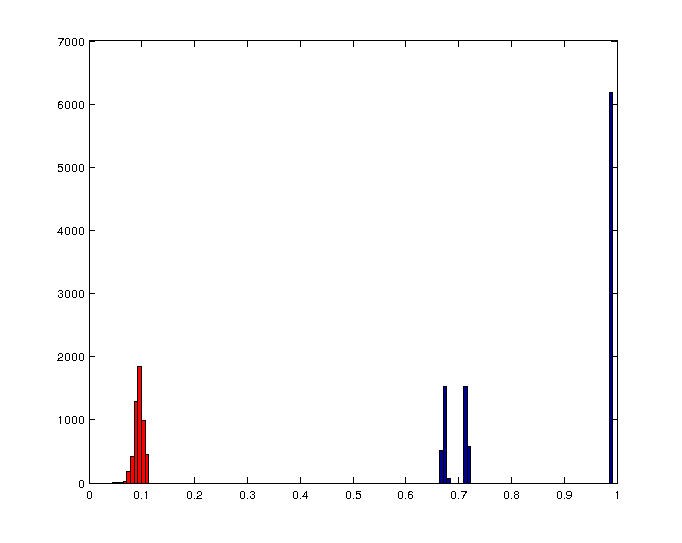
\includegraphics[width=1\textwidth]{ffmpeg-hist}
  \caption{The distribution of the number of differences between original videos (in red) and between original videos and videos processed with ffmpeg (in blue).}\label{fig:ffmpeg-hist}
\end{figure}

The results show that when a video is processed by \emph{Ffmpeg} copying the video stream without re-encoding is enough to greatly alter the file container structure.


\subsection{Exiftool}

\emph{Exiftool} is a command line application for reading, writing and editing metadata information in a variety of media files. With this tool, we have change the creation time information our dataset videos, using the following command:

\begin{lstlisting}
exiftool "-AllDates=1986:11:05 12:00:00" "input.mp4"
\end{lstlisting}

Since we are modifying attributes of the file container that are specific to each unique video, we did not expected this test to perform well. The results are in agreement with this assumption. The changes that \emph{Exiftool} does on a file container are minimal; it just adds a new box at the end of the file, leaving the rest of the structure untouched. As we can see from Fig. \ref{fig:exifaal-hist}, it is not possible to find a threshold that correctly separates the two classes of the binary problem.

\begin{figure}
  \centering
  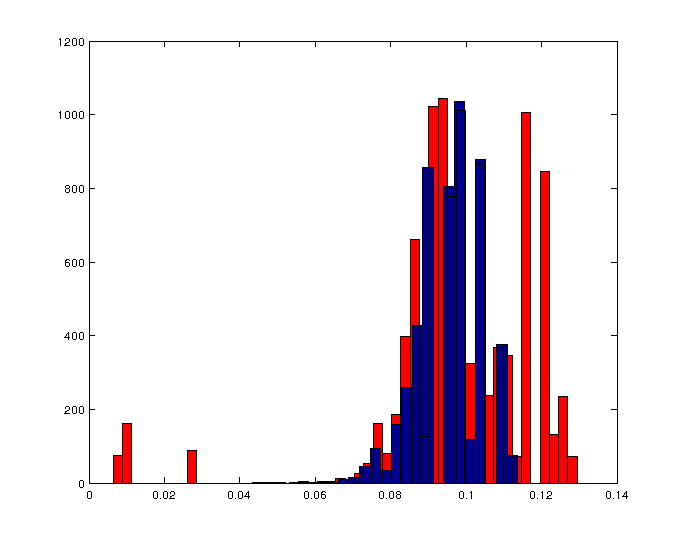
\includegraphics[width=1\textwidth]{exifall-hist}
  \caption{The distribution of the number of differences between original videos (in red) and between original videos and videos processed with exiftool (in blue).}\label{fig:exifaal-hist}
\end{figure}

\begin{figure}
  \centering
  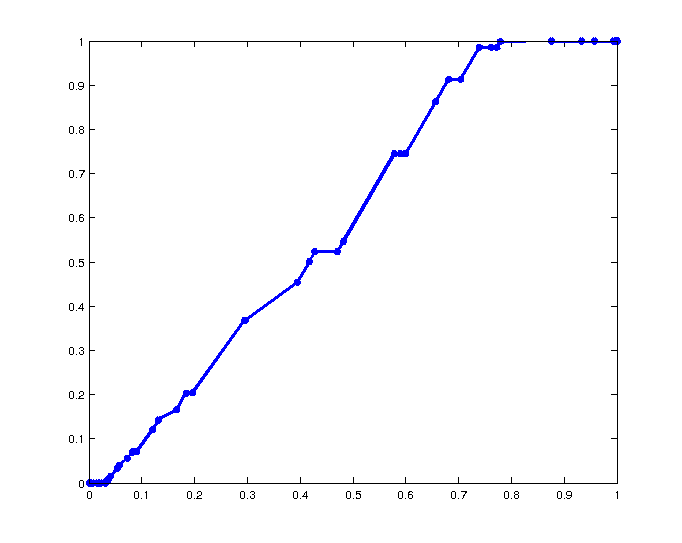
\includegraphics[width=1\textwidth]{exifall-plot}
  \caption{The ROC curve for the experiment with Exiftool shows how the TPR and FPR varies when changing the threshold value.}\label{fig:brand-roc}
\end{figure}

This fact happens because, when we consider all devices, the differences between original videos of the same class for the \emph{Android} devices and for the \emph{iOS} devices have different average values. The additional box that \emph{Exiftool} inserts to the file container for each processed videos adds a constant number of differences for every comparison. This causes the curve associated to the differences between original and processed videos of \emph{Android} devices to overlap the curve associated to the differences between original videos for \emph{iOS} devices.

However, we noticed that the differences between original videos of the same devices regards attributes that are unique to each video, such as \emph{creationTime}, \emph{modificationTime}, \emph{size}, etc. We decided to solve this issue by dynamically build a set composed by attributes whose values are unique to each video for every devices. During the comparison, we will ignore the differences caused by such attributes because their values are not specific to a certain device but to each video.

Without considering such attributes, we are able to separate the two classes with a max accuracy of 1 using a threshold of 0.001.

\section{Source Identification based on File Container}

This section will described the experiments ran to assess the accuracy of our approach with regard to the Source Identification. For each video of the test set we compute the likelihood ratio with respect to every class in the training set. 

When computing the likelihood, the attributes that pertain to the videos and not to the class, as explained previously, will be ignored.

After all the computation have finished, we will obtain a series of likelihood ratios. To each likelihood ratio we need to associate a label accordingly to the class of the test video and the class for which the likelihood have been computed. A label will be 1 the class is the exact brand and model of a test video or is the brand of a test video; it will be 0 otherwise.

Then, using the ROC curve, we determine the threshold value for the likelihood that maximizes the accuracy.

We consider separately the classes that refer to brands and the classes that refer to brands and models, taking into account both manual and automatic mode.

\subsubsection*{Brands}

For manual mode, we obtain a maximum accuracy of 0.98 with a range of likelihood values between a and b, determine using the results from the ROC curve shown in Fig. (ref).

\begin{figure}
  \centering
  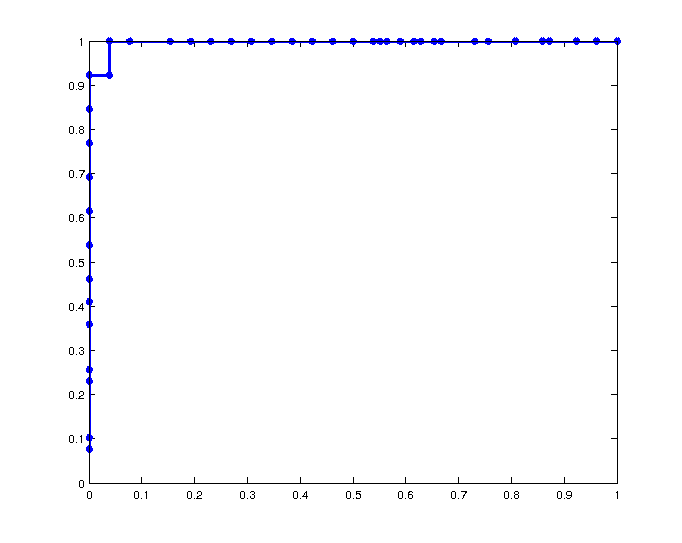
\includegraphics[width=1\textwidth]{brandig-plot}
  \caption{The ROC curve for the experiment with Brands classes shows how the TPR and FPR varies when changing the threshold value.}\label{fig:brand-roc}
\end{figure}

We also determine how precise is the automatic mode by checking the class associated with the higher likelihood ratio. 92\% of the time our method correctly classifies our test videos. For automatic mode, the results can also be visualized in Fig. (ref) where it is shown the confusion matrix. With the confusion matrix we are able to the in which direction the misclassification happened. We can see that the only errors happened because some samsung device are classified as huawei devices. 

\subsubsection*{Brands and Models}

In this case we consider class for which both brand and model are specified. 

For the manual mode, by computing the ROC curve (Fig. \ref{fig:model-roc}, we obtain a maximum accuracy of 0.94 for a range of likelihood values between a and b.

\begin{figure}
  \centering
  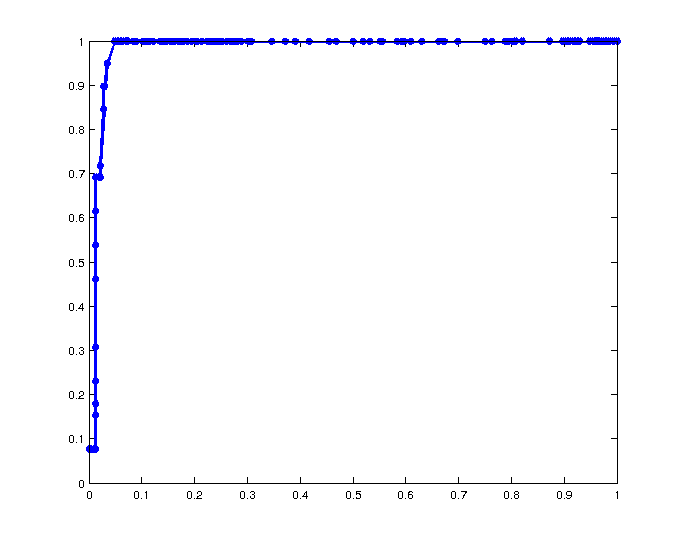
\includegraphics[width=1\textwidth]{modelig-plot}
  \caption{The ROC curve for the experiment with Models classes shows how the TPR and FPR varies when changing the threshold value.}\label{fig:model-roc}
\end{figure}

For the automatic mode, we also determine the precision of our system by computing how many times the correct class is in the top 1 results, in the top 3 results and in the top 5 results. As shown in the table, the correct class is always at least in the top 3 or top 5 and in 84\% of the cases is in the first result.

\section{Application on Social Network}

We have also applied our method to videos that comes from a Social Network, specifically from \emph{Youtube}. The videos of our dataset have been uploaded and then download from \emph{Youtube}.

The experiments have been carried out similarly to the ones for the Integrity Verification. However, we want to determine if videos from \emph{Youtube} are sufficiently similar to be able to distinguish a video that come directly from a source device from a video of that source device that have been subsequently uploaded and downloaded from \emph{Youtube}.

\begin{figure}
  \centering
  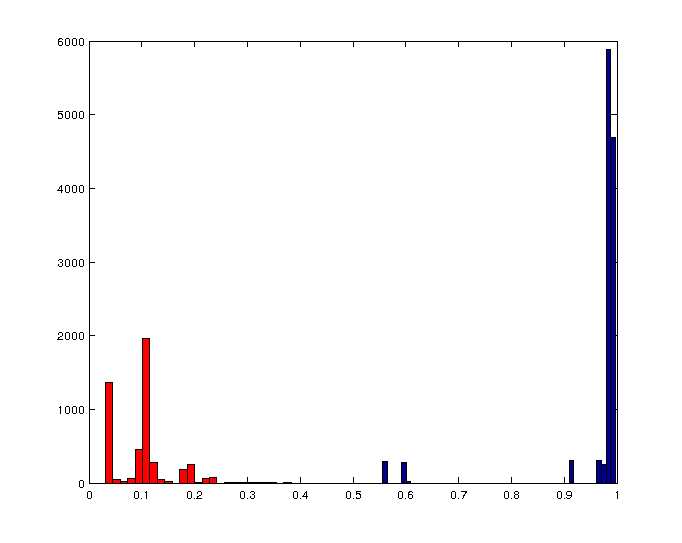
\includegraphics[width=1\textwidth]{youtube-hist}
  \caption{The distribution of the number of differences between \emph{Youtube} videos (in red) and between \emph{Youtube} videos and original videos (in blue).}\label{fig:youtube-hist}
\end{figure}

As can be seen from Fig. \ref{fig:youtube-hist}, the values representing the number of differences between \emph{Youtube} videos and the ones representing the number of differences between original and \emph{Youtube} videos are greatly separated. We obtain a max accuracy of 1 with a range of threshold values between 0.39 and 0.55.



